\begin{figure}[htbp]
\section*{SF3B4}
\centering
\begin{subfigure}[b]{0.95\textwidth}
\centering
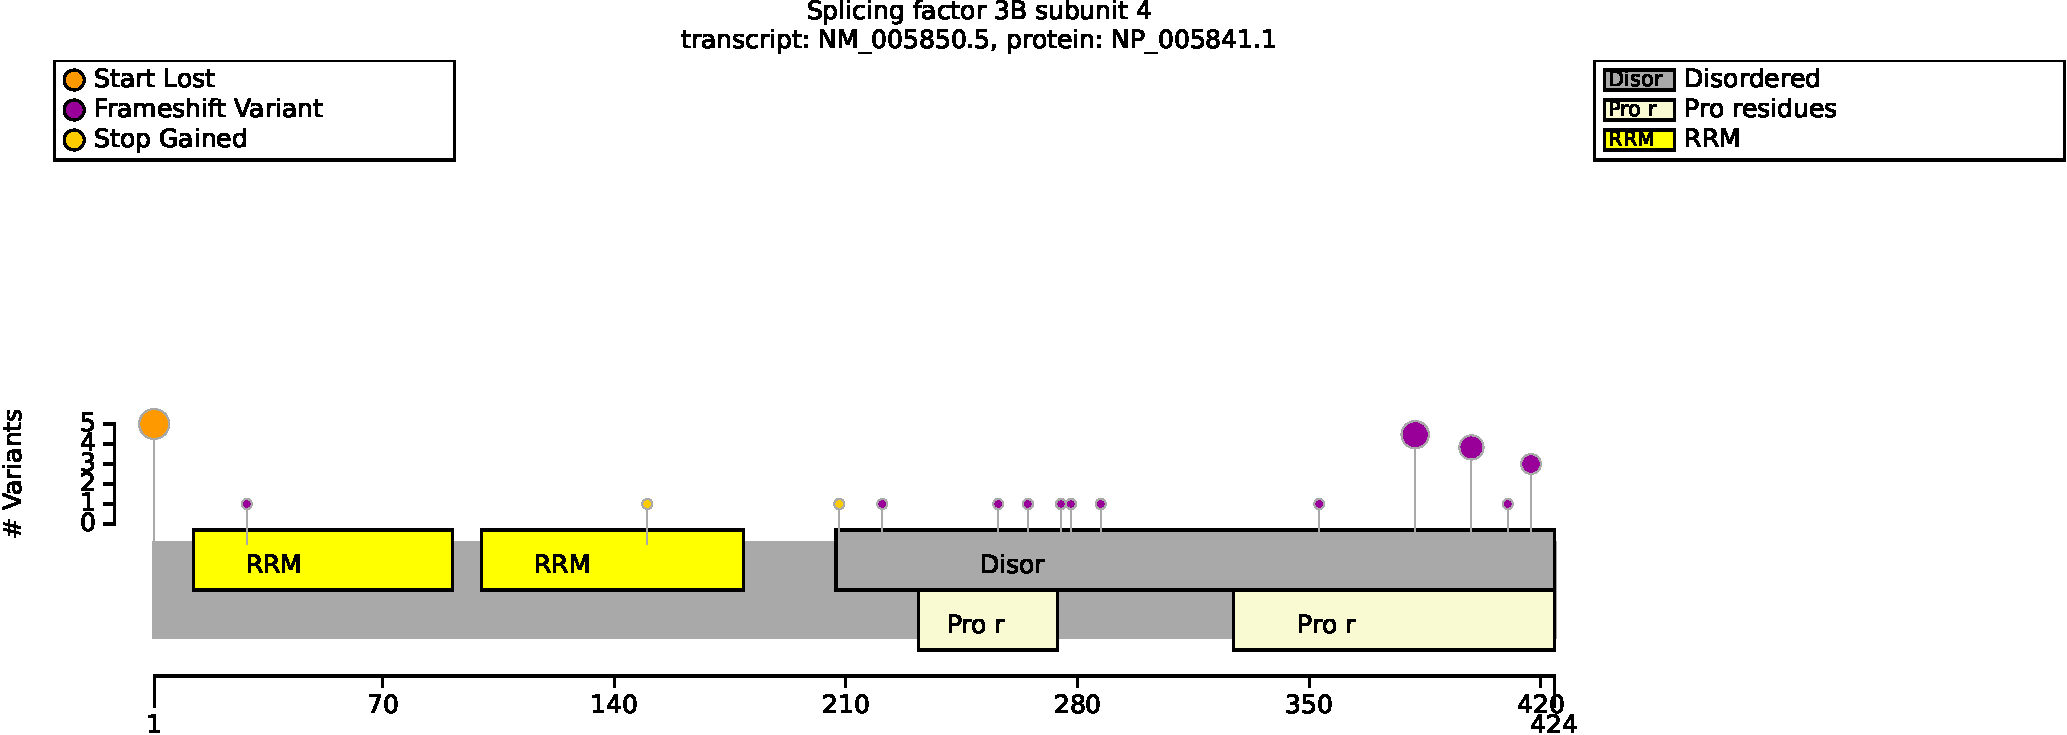
\includegraphics[width=\textwidth]{ img/SF3B4_protein_diagram.pdf} 
\captionsetup{justification=raggedright,singlelinecheck=false}
\caption{Distribution of variants in SF3B4}
\end{subfigure}

\vspace{2em}

\begin{subfigure}[b]{0.95\textwidth}
\centering
\resizebox{\textwidth}{!}{
\begin{tabular}{llllrr}
\toprule
Genotype (A) & Genotype (B) & total tests performed & significant results\\
\midrule
p.Met1? & Other & 37 & 0\\
FEMALE & MALE & 42 & 0\\
\bottomrule
\end{tabular}
}
\captionsetup{justification=raggedright,singlelinecheck=false}
\caption{Fisher Exact Test performed to compare HPO annotation frequency with respect to genotypes.}
\end{subfigure}

\vspace{2em}

\caption{The cohort comprised 26 individuals (18 females, 8 males). A total of 41 HPO terms were used to annotate the cohort. Disease diagnosis: Acrofacial dysostosis 1, Nager type (OMIM:154400). 
In one published analysis, it was stated that ``although no significant genotype–phenotype association was found, it is notable that patients with frameshift SF3B4 variants and predicted to lead to nonsense-mediated RNA 
decay (NMD) of the transcripts tended to have a more severe clinical manifestation''. The authors did not correct for multiple testing and did not find nominally significant associations \cite{PMID_35331022}.
No significant correlation found in our study. A total of 26 unique variant alleles were found in \textit{SF3B4} (transcript: \texttt{NM\_005850.5}, protein id: \texttt{NP\_005841.1}).}
\end{figure}
